\documentclass[tikz,border=3mm]{standalone}
\usepackage{pgfplots}
\pgfplotsset{compat=1.17}
\usepgfplotslibrary{groupplots}
\usetikzlibrary{arrows.meta,positioning,fit,shapes.geometric,calc,backgrounds}
\begin{document}

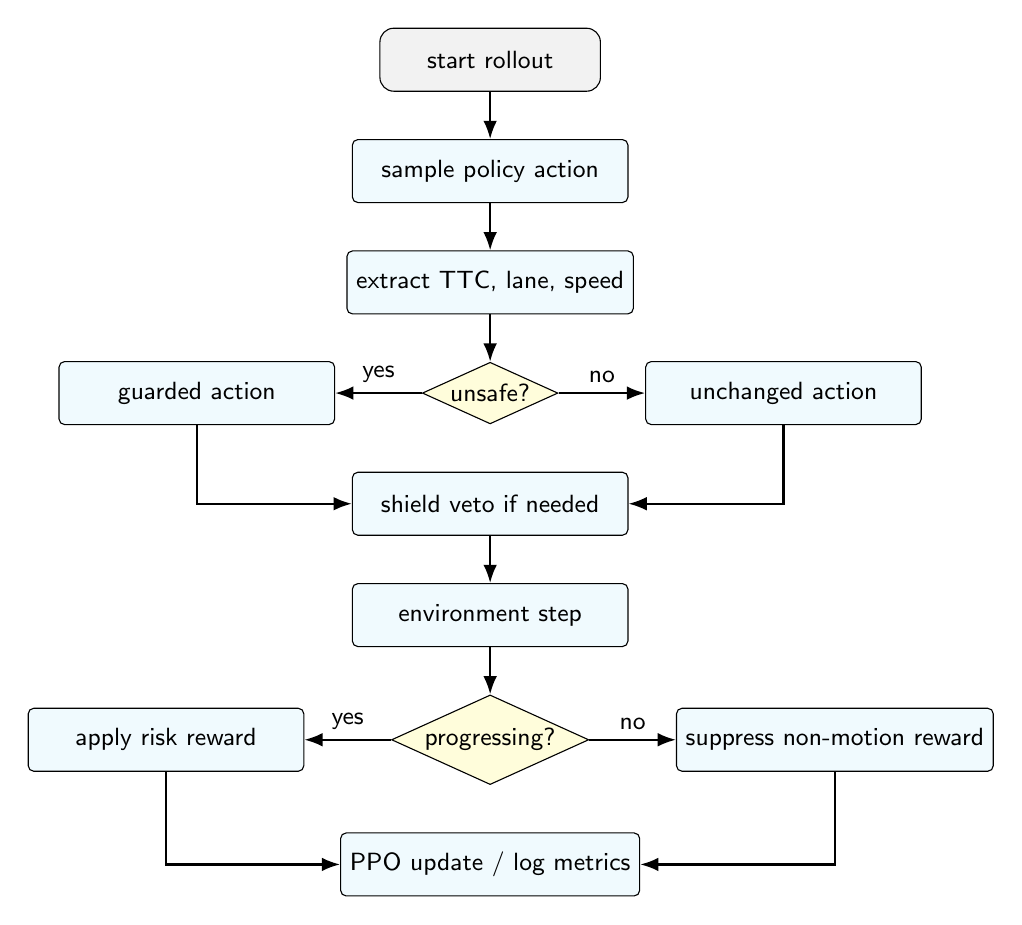
\begin{tikzpicture}[font=\sffamily\small, >=Latex, node distance=6mm and 11mm,
proc/.style={draw, rounded corners=2pt, align=center, minimum width=35mm, minimum height=8mm, fill=cyan!6},
dec/.style={draw, diamond, aspect=2.2, align=center, inner sep=1pt, fill=yellow!14},
term/.style={draw, rounded corners=5pt, align=center, minimum width=28mm, minimum height=8mm, fill=gray!10}]
\node[term] (s) {start rollout};
\node[proc, below=of s] (a) {sample policy action};
\node[proc, below=of a] (x) {extract TTC, lane, speed};
\node[dec, below=of x] (u) {unsafe?};
\node[proc, left=of u] (g) {guarded action};
\node[proc, right=of u] (p) {unchanged action};
\node[proc, below=of u] (v) {shield veto if needed};
\node[proc, below=of v] (e) {environment step};
\node[dec, below=of e] (m) {progressing?};
\node[proc, left=of m] (r) {apply risk reward};
\node[proc, right=of m] (b) {suppress non-motion reward};
\node[proc, below=of m] (upd) {PPO update / log metrics};
\draw[->, thick] (s)--(a); \draw[->, thick] (a)--(x); \draw[->, thick] (x)--(u);
\draw[->, thick] (u)--node[above]{yes}(g); \draw[->, thick] (u)--node[above]{no}(p);
\draw[->, thick] (g)|-(v); \draw[->, thick] (p)|-(v); \draw[->, thick] (v)--(e); \draw[->, thick] (e)--(m);
\draw[->, thick] (m)--node[above]{yes}(r); \draw[->, thick] (m)--node[above]{no}(b);
\draw[->, thick] (r)|-(upd); \draw[->, thick] (b)|-(upd);
\end{tikzpicture}

\end{document}
